\documentclass[10pt,journal,compsoc, twoside]{IEEEtran}

\ifCLASSOPTIONcompsoc
  % IEEE Computer Society needs nocompress option
  % requires cite.sty v4.0 or later (November 2003)
  \usepackage[nocompress]{cite}
\else
  % normal IEEE
  \usepackage{cite}
\fi

\usepackage[left=2cm, top=3cm, right=2cm, bottom=3cm]{geometry}
\usepackage[english]{babel}
\usepackage{graphicx}
\usepackage{amsmath}%
\usepackage{multirow}
\usepackage{xargs}
\usepackage{hyperref}
\usepackage{pgfplots}
\usepackage{listings}
\usepackage{longtable}
\usepackage[usenames,dvipsnames,svgnames,table]{xcolor}
\usepackage{colortbl}
\usepackage{array}
\usepackage{calc}
\usepackage{amssymb}
\usepackage[author={Mathieu}]{pdfcomment}
\usepackage{lipsum}
\usepackage{pifont}
\newcommand{\cmark}{\ding{51}}%
\newcommand{\xmark}{\ding{55}}%


\begin{document}

\title{A New Taxonomy of Bugs Based on the Location of the Correction: An Empirical Study}

\author{

\IEEEauthorblockN{
  Mathieu	Nayrolles\IEEEauthorrefmark{1},
  Abdelwahab Hamou-Lhadj\IEEEauthorrefmark{1},
  Abdou	Maiga\IEEEauthorrefmark{1},
  Alf	Larsson\IEEEauthorrefmark{2},
  Sigrid Eldh\IEEEauthorrefmark{2}}

\IEEEauthorblockA{\vspace{0.2cm}\IEEEauthorrefmark{1}Software Behaviour Analysis (SBA) Research Lab
\\ECE, Concordia University, Montr\'eal, Canada
\\\{m\_nayrol, a\_maiga, abdelw\}@ece.concordia.ca
}
\IEEEauthorblockA{\\\vspace{0.2cm}\IEEEauthorrefmark{2}Ericsson
\\Stockholm, Sweden\\
\{alf.larsson, sigrid.eldh\}@ericsson.com}

}


% make the title area
\maketitle

% As a general rule, do not put math, special symbols or citations
% in the abstract or keywords.
\begin{abstract}
The abstract goes here.
\end{abstract}

% Note that keywords are not normally used for peerreview papers.
\begin{IEEEkeywords}
Bug taxonomy, Bug tracking systems, Empirical studies,
Software maintenance
\end{IEEEkeywords}


\IEEEpeerreviewmaketitle


%!TEX root = bug-taxo.tex

\section{Introduction}

%\IEEEPARstart{T}{his} demo file is intended to serve as a ``starter file''

There have been several studies (e.g., \cite{Weiß2007, Zhang2013}) that study of the factors that influence the bug fixing time.
These studies empirically investigate the relationship between bug report attributes (description, severity, etc.) and the fixing time.
Other studies take bug analysis to another level by investigating techniques and tools for bug prediction and reproduction (e.g., \cite{Chen2013, Kim2007a, Nayrolles2015}).
These studies, however, treat all bugs as being the same.
For example, a bug that requires only one fix is analysed the same way as a bug that necessitates multiple fixes.
Similarly, if multiple bugs are fixed by modifying the exact same locations in the code, then we should investigate how these bugs are related in order to predict them in the future.
Note here that we do not refer to duplicate bugs.
Duplicate bugs are marked as duplicate (and not fixed) and only the master bug is fixed.
As a motivating example, consider Bugs \#AMQ-5066 and \#AMQ-5092 from the Apache Software Foundation bug report management system (used to build one of the datasets in this paper).
Bug \#AMQ-5066 was reported on February 19, 2014 and solved with a patch provided by the reporter.
The solution involves a relatively complex patch that modifies {\tt MQTTProtocolConverter.java}, {\tt MQTTSubscription.java} and {\tt MQTTTest.java} files.
The description of the bug is as follows:
\\ \\
{\it When a client sends a SUBSCRIBE message with the same Topic/Filter as a previous SUBSCRIBE message but a different QoS, the Server MUST discard the older subscription, and resend all retained messages limited to the new Subscription QoS.}
\\ \\
A few months later, another bug, Bug \#AMQ-5092 was reported:
\\ \\
{\it MQTT protocol converters does not correctly generate unique packet ids for retained and non-retained publish messages sent to clients.
[...] Although retained messages published on creation of client subscriptions are copies of retained messages, they must carry a unique packet id when dispatched to clients.
ActiveMQ re-uses the retained message's packet id, which makes it difficult to  acknowledge these messages when wildcard topics are used.
ActiveMQ also sends the same non-retained message multiple times for every matching subscription for overlapping subscriptions.
These messages also re-use the publisher's message id as the packet id, which breaks client acknowledgment.}
\\ \\
This bug was assigned and fixed by a different person than the one who fixed bug \#AMQ-5066.
The fix consists of modifying slightly the same lines of the code in the exact files used to fix Bug \#AMQ-5066.
In fact, Bug \#5092 could have been avoided altogether if the first developer provided a more comprehensive fix to \#AMQ-5066 (a task that is easier said than done).
These two bugs are not duplicates since, according to their description, they deal with different types of problems and yet they can be fixed by providing a similar patch.
In other words, the failures are different while the root causes (faults in the code) are more or less the same.
From the bug handling perspective, if we can develop a way to detect such related bug reports during triaging then we can achieve considerable time saving in the way bug reports are processed, for example, by assigning them to the same developers.
We also conjecture that detecting such related bugs can help with other tasks such as bug reproduction.
We can  reuse the reproduction of an already fixed bug to reproduce an incoming and related bug.

The objective of this paper is not to propose a way to detect such related bug reports or how we can take advantage of them to improve the bug handling process, but it is to introduce a new way of grouping bugs into types that we believe can facilitate the bug handling process.  We are interested in bugs that share similar fixes.
By a fix, we mean a modification (adding or deleting lines of
code) to an exiting file that is used to solve the bug. With this
in mind, the relationship between bugs and fixes can be
modeled using the UML diagram in Figure \ref{fig:bug-taxo-diag}. The diagram
only includes bugs that are fixed. From this figure, we can
think of four instances of this diagram, which we refer to as
bug taxonomy or simply bug types (see Figure \ref{fig:bug-taxo}).

\begin{figure}[h!]
  \centering
    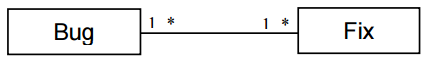
\includegraphics[scale=0.5]{media/bug-taxo-class-diag.png}
    \caption{Class diagram showing the relationship between bugs and fixed
    \label{fig:bug-taxo-diag}}
\end{figure}


\begin{figure}[h!]
  \centering
    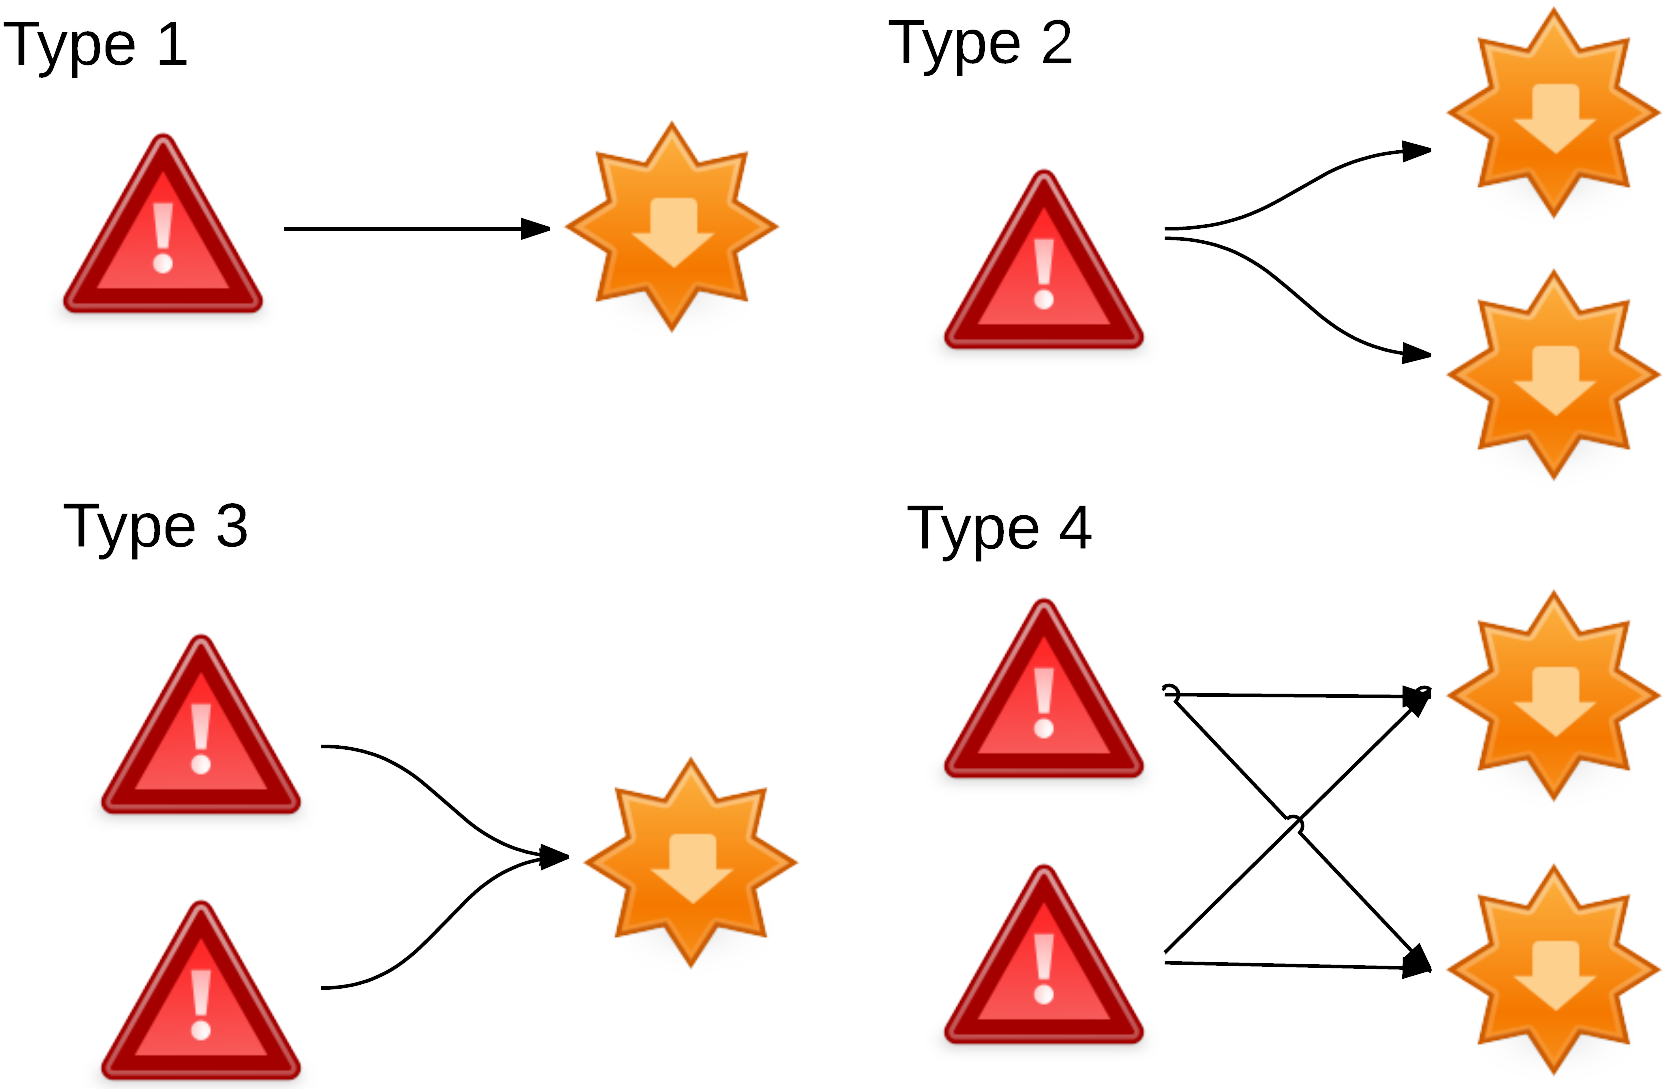
\includegraphics[scale=0.6]{media/bug-taxo.png}
    \caption{Proposed Taxonomy of Bugs
    \label{fig:bug-taxo}}
\end{figure}


The first and second types are the ones we intuitively know
about.
Type 1 refers to a bug being fixed in one single location (i.e., one file), while Type 2 refers to bugs being fixed in more than one location.
In Figure 2, only two locations are shown for the sake of clarity, but many more locations could be involved in the fix of a bug.
Type 3 refers to multiple bugs that are fixed in the exact same location.
Type 4 is an extension of Type 3, where multiple bugs are resolved by modifying the same set of locations.
Note that Type 3 and Type 4 bugs are not duplicates, they may occur when different features of the system fail due to the same root causes (faults).
We conjecture that knowing the proportions of each type of bugs in a system may provide insight into the quality of the system.
Knowing, for example, that in a given system the proportion of Type 2 and 4 bugs is high may be an indication of poor system quality since many fixes are needed to address these bugs.
In addition, the existence of a high number of Types 3 and 4 bugs calls for techniques that can effectively find bug reports related to an incoming bug during triaging.
This is similar to the many studies that exist on detection of duplicates (e.g., \cite{Runeson2007,Sun2010,Nguyen2012}), except that we are not looking for duplicates but for related bugs (bugs that are due to failures of different features of the system, caused by the same faults).
To our knowledge, there is no study that empirically examines bug data with these types in mind, which is the main objective of this section.  By analogy, we can look at the proposed bug taxonomy in a similar way as the clone detection taxonomy presented by Kapser and Godfrey \cite{CoryKapser}. The authors proposed seven types of source code clones and then conducted a case study, using their classification, on the file system module of the Linux operating system. This clone taxonomy continues to be used by researchers to build better approaches for detecting a given clone type and being able to effectively compare approaches with each other.


In this paper,  we are interested in addressing the following research questions:

\begin{itemize}
	\item RQ1: What are the proportions of different types of bugs?
	\item RQ2: How complex is each type of bugs?
	\item RQ3: How pertinent is a bug taxonomy?  [WAHAB: I think you should remove this and keep it for a journal. i suggest to send this paper, without RQ3 to MSR]
\end{itemize}

%!TEX root = bug-taxo.tex

\section{Study Design}

The goal of this study is to analyze the location of bug fixes, with the purpose of classifying bug fixes into types.
More specifically, this study aims to answer the folliwing two research questions:

\begin{itemize}
	\item {\bf RQ$_1$:} {\it What are the proportions of different types of bugs?} This research question aims to what extent bug can be classified according to their fix-locations and the proportion of each types.
  Specifically, we investigate if different types of bugs exists at all and if the proportion of different types in non-negligible.
  As discussed ealier, knowing, for example, that bugs of Type 2 and 4 are the most predominant ones suggests that we need to investigate techniques to help detect whether an incoming bug is of Types 2 and 4 by examining historical data.
  Similarly, if we can automatically identify a bug that is related to another one that has been fixed then we can reuse the results of reproducing the first bug in reproducing the second one.

	\item {\bf RQ$_2$:} {\it How complex is each type of bugs?} This second research question aims to investigate the complexity of the different types of bug.
  More specifically, we analyze and discuss the complexity of different types of bugs using code and process metrics both.
  For the code aspect of the complexity, we compute the number of different files impacted by the fix and the number of hunks and churns.
  We do not compute any statical complexity metrics such as cyclomatic complexity \cite{McCabe1989}.
  For the process aspect of complexity, we analyze the severity of the bug, the amount of duplicate bug report submitted, the number of times a bug report gets reopened, the number of comments and the time required to fix the bug.

\end{itemize}

\subsection{Context Selection}

The context of this study consists of the change history of 388 projects belonging to two software ecosystem, namely, Apache and Netbeans.
Tbale \ref{table:datasets} reports, for each of them, (i) the number of projects analyzed, (ii) size ranges in terms of the number of classes and KLOC, (iii) the overall number of commits and issues analyzed, and (iv) the average, minimum, and maximum length of the projects' story (in years).

\begin{table}[h]
\begin{center}
\begin{tabular}{@{}c|c|c|c|c@{}}
\textbf{Dataset} & \textbf{R/F BR} & \textbf{CS} & \textbf{Files} & \textbf{Projects} \\ \hline \hline
Netbeans         & 53,258          & 122,632     & 30,595         & 39                \\
Apache           & 49,449          & 106,366     & 38,111         & 349               \\
Total            & 102,707         & 229,153     & 68,809         & 388               \\ \hline \hline

\end{tabular}
\end{center}

\caption{Datasets\label{table:datasets}}
\end{table}



All the analysed projects are hosted in {\it Git} or {\it Mercurial} repositories and have either a {\it Jira} or a {\it Bugzilla} issue tracker associated with it.
The Apache ecosystem consists in 349 projects written in various programming languages (C, C++, Java, Python, ...) and uses {\it Git} and {\it Jira}.
These projects represent the Apache ecosystem in its entirety; no system has been excluded from our study.
The complete list can be found online\footnote{https://projects.apache.org/projects.html?name}.
The Netbeans ecosystem consists in 39 projects mostly written in Java.
Similarly to the Apache ecosystem, we did not select some of the projects belonging to the Netbeans ecosystem but all of them.
The Netbeans community uses {\it Bugzilla} and {\it Mercurial}.

The choice of the ecosystems to analyze is not random, but rather driven by the motivation to consider projects having (i) different sizes, (ii) different architectures, and (iii) different development bases and processes.
Indeed, Apache project are extremely various in terms of size of the development team, purpose and technical choices \cite{Bavota2013}.
On the other side, Netbeans have a relatively stable list of core developer and a common vision shared through the 39 related projects \cite{Wang2011}.

Cumulatively, these datasets span from 2001 to 2014. In summary, our consolidated dataset contains 102,707 bugs, 229,153 changesets, 68,809 files that have been modified to fix the bugs, 462,848 comments, and 388 distinct systems.
We also collected 221 million lines of code modified to fix the bugs, identified 3,284 sub-projects, and 17,984 unique contributors to these bug report and source code version management systems.
The cumulated opening time for all the bugs reaches 10,661 working years (3,891,618 working days) which translates into more than one billion dollars\cite{Usnews}.

\subsection{Data Extraction and Analysis}

This subsection describes the data extraction and analysis process that we followed to answer our research questions.

\subsubsection{What are the proportions of different types of bugs?} To answer {\bf RQ$_1$}, we cloned the 349 {\it git} repositories belonging to the Apache ecosystem and the 39 {\it mercurial} repositories belonging to the Netbeans ecosystem.
The raw size of the cloned source code alone, exluding binaries, images and other non-text file, is 163 GB.
Then, we extracted all the 102,707 closed issue that have been resolved using the {\it RESOLVED/FIXED} tags.
Indeed, this study aims to classify bugs according to their fix locations.
If an issue is fixed by other means than {\it fixing} the source code, then, it falls outside the scope our study.
In order to assign commits to issues we used is the regular expression-based approach by Fischer et al. \cite{Fischer} matching the issue ID in the commit note.
Using this technic, we were able to link almost 40\% (40,493 out of 102,707) of our resolved/fixed issues to 229,153 commits.
An issue can be fixed with several commits.

We choose not to use more complex technics like ReLink, an approach proposed by Wu et al.\cite{Wu2011}, which considers the following constraints: (i) matching the committer/authors with issue tracking contributor name/email; (ii) the time interval between the commit and the last comment posted by the same author/contributor on the issue tracker must be less than seven days; and (iii) Vector Space Model (VSM) cosine similarity between the commit note and the last comment referred above or greater than 0.7 because we belive that mining more than forty thousands issues is enough to be significant.

Using our generated consolidated dataset, we extracted the files $f_i$ impacted by each commit $c_i$ for each one of our 388 projects.
Then, we classify the bugs according to the following:

\begin{itemize}
  \item {\bf Type 1:} A bug is tagged type 1 if it is fixed by modifying a file $f_i$ and $f_i$ is not involved in any other bug fix.
  \item {\bf Type 2:} A bug is tagged type 2 if it is fixed by modifying several files $f_{i..n}$ and the files $f_{i..n}$ are not involved in any other bug fix.
  \item {\bf Type 3:} A bug is tagged type 3 if it is fixed by modifying a file $f_{i}$ and the file $f_{i}$ is involved in fixing other bugs.
  \item {\bf Type 4:} A bug is tagged type 4 if it is fixed by modifying several files $f_{i..n}$ and the files $f_{i..n}$ are involved in any other bug fix.
\end{itemize}

To answer this question, we analyze whether any type is predominant in the studied ecosystem, by testing the null hypothesis:

\begin{itemize}
	\item $H_{01A}$ : The proportion of Types does not
change significantly across the studied ecosystems
\end{itemize}

We test this hypothesis by observing both a ``global'' (across ecosystem) and a ``local'' predominance (per ecosystem) of the different types of bugs.
We must observe these two aspects to ensure that the predominance of a particular type of bug is not circumstantial (in few given systems only) but is also not due to some other, unknown factors (in all systems but not in a particular ecosystem).

We answer {\bf RQ$_1$} in two steps.
The first step is to use descriptive statistics; we compute the ratio of each types to the total number of bugs in the dataset.

In the second step, we compare the proportions of the different types of bugs with respect to the ecosystem where the bugs were found.
We build the contingency table with these two qualitative variables (the type and studied ecosystem) and test the null hypothesis {\bf H$_{01A}$} to assess whether the proportion of a particular type of bugs is related to a specific ecosystem or not.

We use the Pearson's chi-squared test to reject the null hypothesis $H_{01A}$.
Pearson's chi-squared independence test is used to analyze the relationship between two qualitative data, in our study the type bugs and the studied ecosystem.
The results of Pearson's chi-squared independence test are considered
statistically significant at $\alpha$ = 0.05.
If p-value $\le$ 0.05, we reject the null hypothesis $H_{01A}$ and conclude that the proportion of each types is different for each ecosystem.

Overall, the data extraction and manipulation for {\bf RQ$_1$} (i.e., cloning repositories, linking commits to issues and tagging issues by type) took thirteen weeks on two Linux servers having 1 quadcore
3.10 GHz CPU and 12 Gb of RAM each.

\subsubsection{How complex is each type of bugs?}  To answer {\bf RQ$_2$} we went through our 40,493 of our resolved/fixed issues and the linked 229,153 commits in order to compute code and process metrics for each of them.
These metrics will then be used to assess the complexity of a bug.
The computed process metrics are:

\begin{itemize}
  \item The time $t$ it took to resolve issue $i$.
  \item The number of issues $dup$ tagged as duplicate of issue $i$.
  \item The number of time issue $i$ got reopen $reop$.
  \item The number of comments $comment$ on issue $i$.
  \item The severity $sev$ of the issue $i$.
\end{itemize}

The computed code metrics are:

\begin{itemize}
  \item The number of files $f$ impacted by issue $i$.
  \item The number of commit $c$ required to fix the issue $i$.
  \item The number of hunks $h$ required to fix the issue $i$.
  \item The number of churns $ch$ required to fix the issue $i$.
\end{itemize}


We address the relation between types and the complexity of the bugs in using our metrics.
We analyze whether Types 2 and 4 bugs are more complex to handle than Types 1 and 3 bugs, by testing the null hypotheses:

\begin{itemize}
 \item  $H_{02S}$ : The severity of different types is not significantly different
 \item  $H_{02D}$ : Different types are not significantly more likely to get duplicated.
 \item  $H_{02R}$ : Different types are not significantly more likely to get reopened.
 \item $H_{02T}$ : There is no statistically-significant difference
between the duration of fixing of different types.
\end{itemize}

For each hypothesis, we build a contingency table with the qualitative variables type of bugs and the dependent variable.

We use the Pearson's chi-squared test to reject the null
hypothesis $H_{02D}$ (respectively $H_{02R}$ ) and $H_{02S}$. The results of Pearson's chi-squared independence test are considered
statistically significant at $\alpha$ = 0.05.
If a p-value $\le$ 0.05, we reject the null hypothesis $H_{02D}$ (respectively $H_{02R}$) andconclude the fact that the bug is more likely to be duplicated (respectively reopened) is related to the type of the bug and we reject $H_{02S}$ and conclude that the severity level of the bug is related to the bug type.

\section{Analysis of the Results}



This section reports the analysis of the results achieved
aiming at answering our two research questions.

\subsection{What are the proportions of different types of bugs?}

% Please add the following required packages to your document preamble:
% \usepackage{multirow}
\begin{table*}[]
\centering
\small
\caption{Contingency table and Pearson's chi-squared tests}
\label{tab:contingency-table}
\begin{tabular}{cccccc}
Ecosystem & T1                 & T2               & T3                & T4                & Pearson's chi-squared p-Value                          \\ \rowcolor{gray!25}
Apache    & 1968  (14.3 \%)   & 1248  (9.1 \%)  & 3101  (22.6 \%)  &7422  ( 54 \%)    &  \\ \rowcolor{gray!25}
Netbeans  & 776  (2.9 \%)     & 240  (0.9 \%)   & 8372  (31.3 \%)  & 17366  (64.9 \%) &  \textless0.01                               \\ \rowcolor{gray!25}
Overall   & 2744  (6.8 \%)    & 1488  (3.7 \%)  & 11473  (28.3 \%) & 24788  (61.2 \%) &                                \\
          & \multicolumn{2}{c}{Types 1 and 2}     & \multicolumn{2}{c}{Types 3 and 4}     &                           \\ \rowcolor{gray!25}
Apache    & \multicolumn{2}{c}{3216  (23.4 \%)}  & \multicolumn{2}{c}{10523  (76.6 \%)} & \\ \rowcolor{gray!25}
Netbeans  & \multicolumn{2}{c}{1016  (3.8 \%)}   & \multicolumn{2}{c}{25738  (96.2 \%)} & \textless0.01                               \\ \rowcolor{gray!25}
All       & \multicolumn{2}{c}{4232  (10.5 \%)}  & \multicolumn{2}{c}{36261  (89.5 \%)} &                                \\
          & \multicolumn{2}{c}{Types 1 and 3}     & \multicolumn{2}{c}{Types 2 and 4}     &                           \\ \rowcolor{gray!25}
Apache    & \multicolumn{2}{c}{5069  (36.9 \%)}  & \multicolumn{2}{c}{8670  (63.1 \%)}  &  \\ \rowcolor{gray!25}
Netbeans  & \multicolumn{2}{c}{9148  (34.2 \%)}  & \multicolumn{2}{c}{17606  (65.8 \%)} &   \textless0.01                             \\ \rowcolor{gray!25}
All       & \multicolumn{2}{c}{14217  (35.1 \%)} & \multicolumn{2}{c}{26276  (64.9 \%)} &
\end{tabular}
\end{table*}


Table \ref{tab:contingency-table} presents a contingency table and the results of the Pearson's chi-squared tests we performed on each types of bug.
In addition to presenting bug types 1 to 4,  Table \ref{tab:contingency-table} also presents regroupement of bug types:
(a) Types 1 and 2 versus Types 3 and 4 and (b) Types 1 and 3 versus Types 2 and 4.


Types 3 (22.6\% and 54\%) and 4 (31.3\% and 64.9\%) are predominants compared to types 1 (14.3\% and 9.1\%) and 2 (6.8\% and 3.7\%) for the Apache and the Netbeans ecosystems, respectively.
Obviously, this observation also holds for when the two ecosystems are combined.
Overall, the proportion of different types of bug is as follows: 6.8\%, 3.7\%, 28.3\%, 61.2\% for types 1, 2, 3 and 4, respectively.
The result of the Pearson's tests are bellow 0.01.
As a reminder, we consider results of Pearson's tests statistically significant at $\alpha \textless0.05$.
Consequently, we can conclude that there is a predominance of Types 3 and 4 in all different ecosystems and this observation is not related to a specific ecosystem.
When combined into our first group, Types 1 \& 2 versus. Types 3 \& 4, there are significantly more Types 3 and 4 (89.5 \%) than Types 1 and 2 (10.5 \%).
In the second group, Types 1 \& 3 versus. Types 2 \& 4, there are significantly more Types 2 \& and 4 (64.9\%) than Types 1 \& 3 (35.1\%).



\subsection{How complex is each type of bugs?}

To answer {\bf RQ$_2$}, we analyse the complexity of each bug in terms of duplication, fixing time, comments, reopenning, files impacted, severity, changesets, hunks and chunks.

Figure \ref{fig:boxplots} presents nine boxplots describing our complexity metric for each types of each ecosystem.
In each sub-figure, the boxplots are organised as follows: (a) Types 1 to 4 of the Apache ecosystem, (b) Types 1 to 4 of the Netbeans ecosystem and (c) Types 1 to 4 of both ecosystems combined.
For all the metrics, except the severity, the median is close to zero and we can observe many outliers.
Tables \ref{tab:apache-eco}, \ref{tab:netbeans-eco} and \ref{tab:overall-eco} present descriptive statistics about each metric for each type for the Apache ecosystem, the Netbeans ecosystem and both ecosystems combined, respectively.
The descriptive Statistics used are $\mu$:mean, $\sum$:sum, $\hat{x}$:median, $\sigma$:standard deviation and $\%$:percentage.
In addition, to the descriptive statistics, these tables present matrixes of Mann-Whitney test for each metric and type.
We added the \checkmark~symbol to the Mann-Whitney test results columns when the value is statistically significant (e.g. $\alpha \textless 0.05$) and \xmark~otherwise.
Tables \ref{tab:combined-one} and \ref{tab:combined-two} are built similarly to Tables \ref{tab:apache-eco}, \ref{tab:netbeans-eco} and \ref{tab:overall-eco} at the exception that they present the data of types groups: Types 1 \& 2 vs. Types 3 \& 4 and Types 1 \& 3 vs. Types 2 \& 4.
Finally, Table \ref{tab:chi-rq2} presents the Pearson's chi-squared tests results for each complexity metrics for Types 1 to 4 and our two types combination.
In what follows, we present our findings for each complexity metric.
omplexity metrics are divided in two groups: (a) process and (b) code metrics.
Process metrics refer to metrics that have been extracted from the project tracking system (i.e. fixing time, comments, reopening and severity).
Code metrics are directly computed using the source code used to fix a given bug (i.e. files impacted, changesets required, hunks and chunks).
We acknowledge that these complexity metrics only represent an abstraction of the actual complexity of a given bug as they cannot account for the actual thought processes and expertise required to craft a fix.
However, we believe that they are an accurate abstraction.
Moreover, they are used in several studies in the field also rely on these metrics to accurately approximate the complexity of bug \cite{Weiß2007,Saha2014,Nam2013,Anvik2006,Nagappan}.

\begin{figure*}
\centering
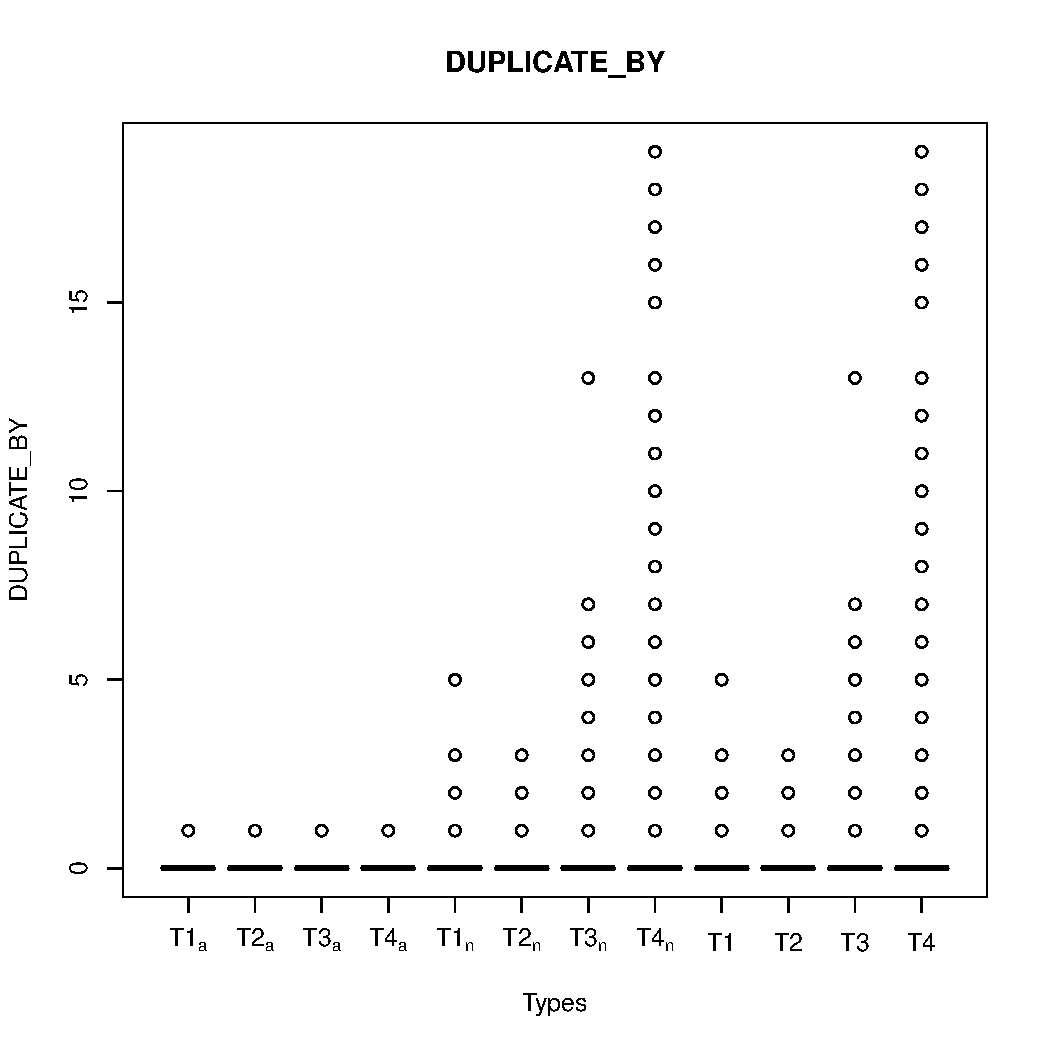
\includegraphics[page=1, width=0.30\textwidth]{extract/Rplots}
\includegraphics[page=2, width=0.30\textwidth]{extract/Rplots}
\includegraphics[page=3, width=0.30\textwidth]{extract/Rplots} \\
\includegraphics[page=4, width=0.30\textwidth]{extract/Rplots}
\includegraphics[page=5, width=0.30\textwidth]{extract/Rplots}
\includegraphics[page=6, width=0.30\textwidth]{extract/Rplots} \\
\includegraphics[page=7, width=0.30\textwidth]{extract/Rplots}
\includegraphics[page=8, width=0.30\textwidth]{extract/Rplots}
\includegraphics[page=9, width=0.30\textwidth]{extract/Rplots}

\caption{Complexity metrics boxplots. From left to right and top to bottom: Duplicate, Fixing time, Comments, Reopening, Files impacted, Severity, Changesets, Hunks and Chunks.
\label{fig:boxplots}}

\end{figure*}


\subsubsection{Duplicate}
The duplicate metric represents the number of time a bug gets resolved using the {\it duplicate} label while referencing one of the {\it resolved/fixed} bug of our dataset.
The process metric is useful to approximate the impact of a given bug on the community.
Indeed, for a bug to be resolved using the {\it duplicate}, it means that the bug has been reported before.
The more a bug gets reported by the community, the more people are impacted enough to report it.
Note that, for a bug$_a$ to be resolved using the {\it duplicate} label and referencing bug$_b$, bug$_b$ does not have to resolved itself.
Indeed, bug$_b$ could be under investigation (i.e. {\it unconfirmed}) or being fixed (i.e. {\it new} or {\it assigned}).

In the Apache ecosystem, the types that are the most likely to get duplicated, ordered by ascending mean duplication rate, are T3 (0.016) $\textless$ T2 (0.022) $\textless$ T1 (0.026) $\textless$ T4 (0.029) and they represent 14.8\%, 8.1\%, 14.5\% and 62.6\% of the total duplications, respectively.
The differences between duplication means by types, however, are only significant in 33.33\% (4/12) of the case.
Indeed, the mean duplication are only significant on the following cases: T1 vs. T3, T3 vs. T4.
For the Apache ecosystem, we can conclude that $T4_{dup}^1 \gg T1_{dup}^2 \gg T3_{dup}^4$.
We use the notation  $x_{m}^r \gg y_{m}^r$ ($x_{m}^r \ll y_{m}^r$) to represent that $x$, along the metric $m$, is significantly greater (lower) than $y$, along the same metric, according to the mann-whitney tests ($\alpha \textless 0.05$).
$r$ represents the rank of $x$ ($y$) according to $m$ from 1 (higher percentage) to 4 (lower percentage).





Netbeans T1 0.086 (2.5\%) T2 0.067 (0.6\%) T3 0.074 (23.3\%) T4 0.113 (73.6\%)

Overall T1 0.043 (3.9\%) T2 0.03 (1.5\%) T3 0.058 (22.3\%) T4 0.088 (72.3\%)

\subsubsection{Fixing time}
\subsubsection{Comments}
\subsubsection{Reopening}
\subsubsection{Severity}
\subsubsection{Files impacted}
\subsubsection{Changesets}
\subsubsection{Hunks}
\subsubsection{Chunks}




%!TEX root = ..bug-taxo.tex

% Please add the following required packages to your document preamble:
% \usepackage{graphicx}
\begin{table*}[]
\centering
\samll
\setlength\extrarowheight{6pt}
\caption{My caption}
\label{my-label}
\begin{tabular}{ccccccc|ccccc}

Types & Metric &$^\mu$ & $^\sum$ & $^\hat{x}$ & $^\sigma$ & $^\%$ & T1 & T2 & T3 & T4 \\ \hline \rowcolor{gray!25}
& Dup. & 0.026 & 51 & 0 & 0.2 & 14.8 & n.a & \xmark (0.53) & \checkmark  (\textless 0.05) & \xmark (0.45)  \\ \rowcolor{gray!25}
& Tim. & 91.574 & 180217 & 4 & 262 & 21.8 & n.a & \checkmark  (\textless 0.05) & \checkmark  (\textless 0.05) & \checkmark  (\textless 0.05)  \\ \rowcolor{gray!25}
& Com. & 4.355 & 8571 & 3 & 4.7 & 9.5 & n.a & \checkmark  (\textless 0.05) & \xmark (0.17) & \checkmark  (\textless 0.05)  \\ \rowcolor{gray!25}
& Reo. & 0.062 & 122 & 0 & 0.3 & 13.8 & n.a & \xmark (0.29) & \checkmark  (\textless 0.05) & \checkmark  (\textless 0.05)  \\ \rowcolor{gray!25}
T1 & Fil. & 0.991 & 1950 & 1 & 0.1 & 3.7 & n.a & \checkmark  (\textless 0.05) & \xmark (0.28) & \checkmark  (\textless 0.05)  \\ \rowcolor{gray!25}
& Sev. & 3.423 & 6737 & 4 & 1.3 & 13.2 & n.a & \xmark (0.18) & \checkmark  (\textless 0.05) & \checkmark  (\textless 0.05)  \\ \rowcolor{gray!25}
& Cha. & 1 & 1968 & 1 & 0 & 1.9 & n.a & \checkmark  (\textless 0.05) & \checkmark  (\textless 0.05) & \checkmark  (\textless 0.05)  \\ \rowcolor{gray!25}
& Hun. & 3.814 & 7506 & 3 & 2.4 & 0 & n.a & \checkmark  (\textless 0.05) & \checkmark  (\textless 0.05) & \checkmark  (\textless 0.05)  \\ \rowcolor{gray!25}
& Chur. & 18.761 & 36921 & 7 & 48.6 & 0 & n.a & \checkmark  (\textless 0.05) & \xmark (0.09) & \checkmark  (\textless 0.05)  \\


 & Dup. & 0.022 & 28 & 0 & 0.1 & 8.1 & \xmark (0.53) & n.a & \xmark (0.16) & \xmark (0.19)  \\
 & Tim. & 115.158 & 143717 & 8 & 294.1 & 17.4 & \checkmark  (\textless 0.05) & n.a & \checkmark  (\textless 0.05) & \checkmark  (\textless 0.05)  \\
 & Com. & 5.041 & 6291 & 4 & 4.7 & 7 & \checkmark  (\textless 0.05) & n.a & \checkmark  (\textless 0.05) & \checkmark  (\textless 0.05)  \\
 & Reo. & 0.071 & 89 & 0 & 0.3 & 10.1 & \xmark (0.29) & n.a & \checkmark  (\textless 0.05) & \xmark (0.59)  \\
T2 & Fil. & 4.381 & 5468 & 2 & 20.4 & 10.5 & \checkmark  (\textless 0.05) & n.a & \checkmark  (\textless 0.05) & \checkmark  (\textless 0.05)  \\
 & Sev. & 3.498 & 4365 & 4 & 1.2 & 8.6 & \xmark (0.18) & n.a & \checkmark  (\textless 0.05) & \checkmark  (\textless 0.05)  \\
 & Cha. & 4.681 & 5842 & 2 & 20.4 & 5.5 & \checkmark  (\textless 0.05) & n.a & \checkmark  (\textless 0.05) & \checkmark  (\textless 0.05)  \\
 & Hun. & 561.995 & 701370 & 14 & 13628.2 & 3.9 & \checkmark  (\textless 0.05) & n.a & \checkmark  (\textless 0.05) & \checkmark  (\textless 0.05)  \\
 & Chur. & 14184.869 & 17702716 & 88 & 400710.2 & 8 & \checkmark  (\textless 0.05) & n.a & \checkmark  (\textless 0.05) & \checkmark  (\textless 0.05)  \\

 \rowcolor{gray!25}
 & Dup. & 0.016 & 50 & 0 & 0.1 & 14.5 & \checkmark  (\textless 0.05) & \xmark (0.16) & n.a & \checkmark  (\textless 0.05)  \\ \rowcolor{gray!25}
 & Tim. & 35.892 & 111300 & 1 & 151.8 & 13.5 & \checkmark  (\textless 0.05) & \checkmark  (\textless 0.05) & n.a & \checkmark  (\textless 0.05)  \\ \rowcolor{gray!25}
 & Com. & 4.422 & 13712 & 3 & 4.4 & 15.2 & \xmark (0.17) & \checkmark  (\textless 0.05) & n.a & \checkmark  (\textless 0.05)  \\ \rowcolor{gray!25}
 & Reo. & 0.033 & 101 & 0 & 0.2 & 11.5 & \checkmark  (\textless 0.05) & \checkmark  (\textless 0.05) & n.a & \checkmark  (\textless 0.05)  \\ \rowcolor{gray!25}
 T3 & Fil. & 0.994 & 3081 & 1 & 0.1 & 5.9 & \xmark (0.28) & \checkmark  (\textless 0.05) & n.a & \checkmark  (\textless 0.05)  \\ \rowcolor{gray!25}
 & Sev. & 3.644 & 11300 & 4 & 1.1 & 22.2 & \checkmark  (\textless 0.05) & \checkmark  (\textless 0.05) & n.a & \checkmark  (\textless 0.05)  \\ \rowcolor{gray!25}
 & Cha. & 1 & 3101 & 1 & 0 & 2.9 & \checkmark  (\textless 0.05) & \checkmark  (\textless 0.05) & n.a & \checkmark  (\textless 0.05)  \\ \rowcolor{gray!25}
 & Hun. & 4.022 & 12472 & 3 & 3.4 & 0.1 & \checkmark  (\textless 0.05) & \checkmark  (\textless 0.05) & n.a & \checkmark  (\textless 0.05)  \\ \rowcolor{gray!25}
 & Chur. & 16.954 & 52573 & 6 & 49.8 & 0 & \xmark (0.09) & \checkmark  (\textless 0.05) & n.a & \checkmark  (\textless 0.05)  \\


& Dup. & 0.029 & 216 & 0 & 0.2 & 62.6 & \xmark (0.45) & \xmark (0.19) & \checkmark  (\textless 0.05) & n.a  \\
& Tim. & 52.76 & 391586 & 4 & 182.2 & 47.4 & \checkmark  (\textless 0.05) & \checkmark  (\textless 0.05) & \checkmark  (\textless 0.05) & n.a  \\
& Com. & 8.313 & 61701 & 5 & 10.2 & 68.3 & \checkmark  (\textless 0.05) & \checkmark  (\textless 0.05) & \checkmark  (\textless 0.05) & n.a  \\
& Reo. & 0.077 & 570 & 0 & 0.3 & 64.6 & \checkmark  (\textless 0.05) & \xmark (0.59) & \checkmark  (\textless 0.05) & n.a  \\
T4 & Fil. & 5.633 & 41805 & 3 & 14 & 79.9 & \checkmark  (\textless 0.05) & \checkmark  (\textless 0.05) & \checkmark  (\textless 0.05) & n.a  \\
& Sev. & 3.835 & 28466 & 4 & 1 & 56 & \checkmark  (\textless 0.05) & \checkmark  (\textless 0.05) & \checkmark  (\textless 0.05) & n.a  \\
& Cha. & 12.861 & 95455 & 4 & 52.2 & 89.7 & \checkmark  (\textless 0.05) & \checkmark  (\textless 0.05) & \checkmark  (\textless 0.05) & n.a  \\
& Hun. & 2305.868 & 17114149 & 30 & 58094.7 & 96 & \checkmark  (\textless 0.05) & \checkmark  (\textless 0.05) & \checkmark  (\textless 0.05) & n.a  \\
& Chur. & 27249.773 & 202247816 & 204 & 320023.5 & 91.9 & \checkmark  (\textless 0.05) & \checkmark  (\textless 0.05) & \checkmark  (\textless 0.05) & n.a

\end{tabular}%
\end{table*}

%!TEX root = ..bug-taxo.tex

\begin{table*}[]
\centering
\small
\setlength\extrarowheight{6pt}
\caption{My caption}
\label{my-label}
\begin{tabular}{ccccccc|ccccc}

Types & Metric &$^\mu$ & $^\sum$ & $^\hat{x}$ & $^\sigma$ & $^\%$ & T1 & T2 & T3 & T4 \\ \hline \rowcolor{gray!25}

& Dup. & 0.086 & 67 & 0 & 0.4 & 2.5 & n.a & \xmark (0.39) & \xmark (0.24) & \xmark (0.86) \\  \rowcolor{gray!25}
& Tim. & 92.759 & 71981 & 10 & 219.1 & 2.3 & n.a & \checkmark  (\textless 0.05) & \xmark (0.15) & \checkmark  (\textless 0.05) \\  \rowcolor{gray!25}
& Com. & 4.687 & 3637 & 3 & 4.1 & 2.4 & n.a & \checkmark  (\textless 0.05) & \xmark (0.83) & \checkmark  (\textless 0.05)  \\  \rowcolor{gray!25}
& Reo. & 0.054 & 42 & 0 & 0.3 & 1.9 & n.a & \xmark (0.1) & \xmark (0.58) & \checkmark  (\textless 0.05)  \\  \rowcolor{gray!25}
T1 & Fil. & 1.735 & 1346 & 1 & 13.2 & 0.8 & n.a & \checkmark  (\textless 0.05) & \checkmark  (\textless 0.05) & \checkmark  (\textless 0.05)  \\  \rowcolor{gray!25}
& Sev. & 4.314 & 3348 & 3 & 1.5 & 3.1 & n.a & \xmark (0.66) & \checkmark  (\textless 0.05) & \checkmark  (\textless 0.05)  \\  \rowcolor{gray!25}
& Cha. & 1.085 & 842 & 1 & 0.4 & 2 & n.a & \xmark (0.99) & \xmark (0.26) & \checkmark  (\textless 0.05)  \\  \rowcolor{gray!25}
& Hun. & 4.405 & 3418 & 3 & 7 & 0.5 & n.a & \checkmark  (\textless 0.05) & \xmark (0.13) & \checkmark  (\textless 0.05)  \\  \rowcolor{gray!25}
& Chur. & 5.089 & 3949 & 2 & 12.5 & 0.3 & n.a & \checkmark  (\textless 0.05) & \checkmark  (\textless 0.05) & \checkmark  (\textless 0.05)  \\


 & Dup. & 0.067 & 16 & 0 & 0.3 & 0.6 & \xmark (0.39) & n.a & \xmark (0.73) & \xmark (0.39) \\
 & Tim. & 111.9 & 26856 & 16 & 308.6 & 0.9 & \checkmark  (\textless 0.05) & n.a & \checkmark  (\textless 0.05) & \xmark (0.41) \\
 & Com. & 4.433 & 1064 & 3 & 4 & 0.7 & \checkmark  (\textless 0.05) & n.a & \checkmark  (\textless 0.05) & \checkmark  (\textless 0.05) \\
 & Reo. & 0.079 & 19 & 0 & 0.3 & 0.9 & \xmark (0.1) & n.a & \xmark (0.11) & \xmark (0.97) \\
T2 & Fil. & 8.804 & 2113 & 2 & 42.7 & 1.3 & \checkmark  (\textless 0.05) & n.a & \checkmark  (\textless 0.05) & \checkmark  (\textless 0.05) \\
 & Sev. & 4.362 & 1047 & 3 & 1.5 & 1 & \xmark (0.66) & n.a & \checkmark  (\textless 0.05) & \checkmark  (\textless 0.05) \\
 & Cha. & 1.075 & 258 & 1 & 0.3 & 0.6 & \xmark (0.99) & n.a & \xmark (0.5) & \checkmark  (\textless 0.05)  \\
 & Hun. & 21.887 & 5253 & 8 & 62.7 & 0.7 & \checkmark  (\textless 0.05) & n.a & \checkmark  (\textless 0.05) & \checkmark  (\textless 0.05) \\
 & Chur. & 32.263 & 7743 & 8 & 125.8 & 0.7 & \checkmark  (\textless 0.05) & n.a & \checkmark  (\textless 0.05) & \checkmark  (\textless 0.05)  \\

 \rowcolor{gray!25}
& Dup. & 0.074 & 620 & 0 & 0.4 & 23.3 & \xmark (0.24) & \xmark (0.73) & n.a & \checkmark  (\textless 0.05)  \\  \rowcolor{gray!25}
& Tim. & 87.033 & 728642 & 9 & 233.6 & 23.8 & \xmark (0.15) & \checkmark  (\textless 0.05) & n.a & \checkmark  (\textless 0.05) \\  \rowcolor{gray!25}
& Com. & 4.73 & 39599 & 3 & 4.3 & 26.5 & \xmark (0.83) & \checkmark  (\textless 0.05) & n.a & \checkmark  (\textless 0.05)  \\  \rowcolor{gray!25}
& Reo. & 0.06 & 499 & 0 & 0.3 & 22.7 & \xmark (0.58) & \xmark (0.11) & n.a & \checkmark  (\textless 0.05)  \\  \rowcolor{gray!25}
T3 & Fil. & 1.306 & 10932 & 1 & 5.1 & 6.8 & \checkmark  (\textless 0.05) & \checkmark  (\textless 0.05) & n.a & \checkmark  (\textless 0.05) \\  \rowcolor{gray!25}
& Sev. & 4.021 & 33666 & 3 & 1.4 & 31.4 & \checkmark  (\textless 0.05) & \checkmark  (\textless 0.05) & n.a & \checkmark  (\textless 0.05) \\  \rowcolor{gray!25}
& Cha. & 1.065 & 8917 & 1 & 0.3 & 21 & \xmark (0.26) & \xmark (0.5) & n.a & \checkmark  (\textless 0.05) \\  \rowcolor{gray!25}
& Hun. & 5.15 & 43115 & 3 & 12.4 & 5.8 & \xmark (0.13) & \checkmark  (\textless 0.05) & n.a & \checkmark  (\textless 0.05) \\  \rowcolor{gray!25}
& Chur. & 6.727 & 56317 & 2 & 22 & 4.9 & \checkmark  (\textless 0.05) & \checkmark  (\textless 0.05) & n.a & \checkmark  (\textless 0.05)  \\


 & Dup. & 0.113 & 1959 & 0 & 0.7 & 73.6 & \xmark (0.86) & \xmark (0.39) & \checkmark  (\textless 0.05) & n.a \\
 & Tim. & 128.833 & 2237319 & 13 & 332.8 & 73 & \checkmark  (\textless 0.05) & \xmark (0.41) & \checkmark  (\textless 0.05) & n.a \\
 & Com. & 6.058 & 105202 & 4 & 6.7 & 70.4 & \checkmark  (\textless 0.05) & \checkmark  (\textless 0.05) & \checkmark  (\textless 0.05) & n.a \\
 & Reo. & 0.094 & 1639 & 0 & 0.4 & 74.5 & \checkmark  (\textless 0.05) & \xmark (0.97) & \checkmark  (\textless 0.05) & n.a & \\
T4 & Fil. & 8.408 & 146019 & 4 & 25.1 & 91 & \checkmark  (\textless 0.05) & \checkmark  (\textless 0.05) & \checkmark  (\textless 0.05) & n.a \\
 & Sev. & 3.982 & 69159 & 3 & 1.4 & 64.5 & \checkmark  (\textless 0.05) & \checkmark  (\textless 0.05) & \checkmark  (\textless 0.05) & n.a \\
 & Cha. & 1.871 & 32494 & 2 & 1.2 & 76.4 & \checkmark  (\textless 0.05) & \checkmark  (\textless 0.05) & \checkmark  (\textless 0.05) & n.a \\
 & Hun. & 40.195 & 698022 & 13 & 98.3 & 93.1 & \checkmark  (\textless 0.05) & \checkmark  (\textless 0.05) & \checkmark  (\textless 0.05) & n.a  \\
 & Chur. & 61.893 & 1074830 & 15 & 178.6 & 94 & \checkmark  (\textless 0.05) & \checkmark  (\textless 0.05) & \checkmark  (\textless 0.05) & n.a

\end{tabular}%
\end{table*}

%!TEX root = ..bug-taxo.tex

\begin{table*}[]
\centering
\samll
\setlength\extrarowheight{6pt}
\caption{My caption}
\label{my-label}
\begin{tabular}{ccccccc|ccccc}

Types & Metric &$^\mu$ & $^\sum$ & $^\hat{x}$ & $^\sigma$ & $^\%$ & T1 & T2 & T3 & T4 \\ \hline \rowcolor{gray!25}
& Dup. & 0.043 & 118 & 0 & 0.3 & 3.9 & n.a & \xmark (0.09) & \xmark (0.16) & \checkmark  (\textless 0.05)  \\  \rowcolor{gray!25}
& Tim. & 91.909 & 252198 & 6 & 250.6 & 6.5 & n.a & \checkmark  (\textless 0.05) & \checkmark  (\textless 0.05) & \checkmark  (\textless 0.05)  \\  \rowcolor{gray!25}
& Com. & 4.449 & 12208 & 3 & 4.5 & 5.1 & n.a & \checkmark  (\textless 0.05) & \checkmark  (\textless 0.05) & \checkmark  (\textless 0.05)  \\  \rowcolor{gray!25}
& Reo. & 0.06 & 164 & 0 & 0.3 & 5.3 & n.a & \xmark (0.07) & \checkmark  (\textless 0.05) & \checkmark  (\textless 0.05)  \\  \rowcolor{gray!25}
T1 & Fil. & 1.201 & 3296 & 1 & 7 & 1.5 & n.a & \checkmark  (\textless 0.05) & \checkmark  (\textless 0.05) & \checkmark  (\textless 0.05)  \\  \rowcolor{gray!25}
& Sev. & 3.675 & 10085 & 4 & 1.4 & 6.4 & n.a & \xmark (0.97) & \xmark (0.17) & \checkmark  (\textless 0.05)  \\  \rowcolor{gray!25}
& Cha. & 1.024 & 2810 & 1 & 0.2 & 1.9 & n.a & \checkmark  (\textless 0.05) & \checkmark  (\textless 0.05) & \checkmark  (\textless 0.05)  \\  \rowcolor{gray!25}
& Hun. & 3.981 & 10924 & 3 & 4.3 & 0.1 & n.a & \checkmark  (\textless 0.05) & \checkmark  (\textless 0.05) & \checkmark  (\textless 0.05)  \\  \rowcolor{gray!25}
& Chur. & 14.894 & 40870 & 5 & 42.2 & 0 & n.a & \checkmark  (\textless 0.05) & \checkmark  (\textless 0.05) & \checkmark  (\textless 0.05)  \\


& Dup. & 0.03 & 44 & 0 & 0.2 & 1.5 & \xmark (0.09) & n.a & \checkmark  (\textless 0.05) & \checkmark  (\textless 0.05)  \\
& Tim. & 114.632 & 170573 & 9 & 296.4 & 4.4 & \checkmark  (\textless 0.05) & n.a & \checkmark  (\textless 0.05) & \xmark (0.15)  \\
& Com. & 4.943 & 7355 & 3 & 4.6 & 3.1 & \checkmark  (\textless 0.05) & n.a & \xmark (0.72) & \checkmark  (\textless 0.05)  \\
& Reo. & 0.073 & 108 & 0 & 0.3 & 3.5 & \xmark (0.07) & n.a & \checkmark  (\textless 0.05) & \xmark (0.47)  \\
T2 & Fil. & 5.095 & 7581 & 2 & 25.4 & 3.6 & \checkmark  (\textless 0.05) & n.a & \checkmark  (\textless 0.05) & \checkmark  (\textless 0.05)  \\
& Sev. & 3.637 & 5412 & 4 & 1.3 & 3.4 & \xmark (0.97) & n.a & \xmark (0.44) & \xmark (0.1)  \\
& Cha. & 4.099 & 6100 & 2 & 18.7 & 4.1 & \checkmark  (\textless 0.05) & n.a & \checkmark  (\textless 0.05) & \checkmark  (\textless 0.05)  \\
& Hun. & 474.881 & 706623 & 12 & 12481.7 & 3.8 & \checkmark  (\textless 0.05) & n.a & \checkmark  (\textless 0.05) & \checkmark  (\textless 0.05)  \\
& Chur. & 11902.19 & 17710459 & 62 & 366988 & 8 & \checkmark  (\textless 0.05) & n.a & \checkmark  (\textless 0.05) & \checkmark  (\textless 0.05)  \\

 \rowcolor{gray!25}
& Dup. & 0.058 & 670 & 0 & 0.4 & 22.3 & \xmark (0.16) & \checkmark  (\textless 0.05) & n.a & \checkmark  (\textless 0.05)  \\  \rowcolor{gray!25}
& Tim. & 73.21 & 839942 & 6 & 215.8 & 21.6 & \checkmark  (\textless 0.05) & \checkmark  (\textless 0.05) & n.a & \checkmark  (\textless 0.05)  \\  \rowcolor{gray!25}
& Com. & 4.647 & 53311 & 3 & 4.3 & 22.2 & \checkmark  (\textless 0.05) & \xmark (0.72) & n.a & \checkmark  (\textless 0.05)  \\  \rowcolor{gray!25}
& Reo. & 0.052 & 600 & 0 & 0.3 & 19.5 & \checkmark  (\textless 0.05) & \checkmark  (\textless 0.05) & n.a & \checkmark  (\textless 0.05)  \\  \rowcolor{gray!25}
T3 & Fil. & 1.221 & 14013 & 1 & 4.4 & 6.6 & \checkmark  (\textless 0.05) & \checkmark  (\textless 0.05) & n.a & \checkmark  (\textless 0.05)  \\  \rowcolor{gray!25}
& Sev. & 3.919 & 44966 & 3 & 1.4 & 28.4 & \xmark (0.17) & \xmark (0.44) & n.a & \checkmark  (\textless 0.05)  \\  \rowcolor{gray!25}
& Cha. & 1.048 & 12018 & 1 & 0.3 & 8.1 & \checkmark  (\textless 0.05) & \checkmark  (\textless 0.05) & n.a & \checkmark  (\textless 0.05)  \\  \rowcolor{gray!25}
& Hun. & 4.845 & 55587 & 3 & 10.7 & 0.3 & \checkmark  (\textless 0.05) & \checkmark  (\textless 0.05) & n.a & \checkmark  (\textless 0.05)  \\  \rowcolor{gray!25}
& Chur. & 9.491 & 108890 & 3 & 32.3 & 0 & \checkmark  (\textless 0.05) & \checkmark  (\textless 0.05) & n.a & \checkmark  (\textless 0.05)  \\


& Dup. & 0.088 & 2175 & 0 & 0.6 & 72.3 & \checkmark  (\textless 0.05) & \checkmark  (\textless 0.05) & \checkmark  (\textless 0.05) & n.a  \\
& Tim. & 106.056 & 2628905 & 9 & 297.9 & 67.6 & \checkmark  (\textless 0.05) & \xmark (0.15) & \checkmark  (\textless 0.05) & n.a  \\
& Com. & 6.733 & 166903 & 4 & 8 & 69.6 & \checkmark  (\textless 0.05) & \checkmark  (\textless 0.05) & \checkmark  (\textless 0.05) & n.a  \\
& Reo. & 0.089 & 2209 & 0 & 0.4 & 71.7 & \checkmark  (\textless 0.05) & \xmark (0.47) & \checkmark  (\textless 0.05) & n.a  \\
T4 & Fil. & 7.577 & 187824 & 3 & 22.4 & 88.3 & \checkmark  (\textless 0.05) & \checkmark  (\textless 0.05) & \checkmark  (\textless 0.05) & n.a  \\
& Sev. & 3.938 & 97625 & 3 & 1.3 & 61.8 & \checkmark  (\textless 0.05) & \xmark (0.1) & \checkmark  (\textless 0.05) & n.a  \\
& Cha. & 5.162 & 127949 & 2 & 29 & 85.9 & \checkmark  (\textless 0.05) & \checkmark  (\textless 0.05) & \checkmark  (\textless 0.05) & n.a  \\
& Hun. & 718.58 & 17812171 & 16 & 31804.5 & 95.8 & \checkmark  (\textless 0.05) & \checkmark  (\textless 0.05) & \checkmark  (\textless 0.05) & n.a  \\
& Chur. & 8202.463 & 203322646 & 28 & 175548.3 & 91.9 & \checkmark  (\textless 0.05) & \checkmark  (\textless 0.05) & \checkmark  (\textless 0.05) & n.a
\end{tabular}%
\end{table*}

%!TEX root = ..bug-taxo.tex

% Please add the following required packages to your document preamble:
% \usepackage{multirow}
% \usepackage{graphicx}

\definecolor{Gray}{gray}{0.85}
\begin{table*}[]
\small
\centering
\setlength\extrarowheight{8pt}
\caption{My caption}
\label{my-label}
\resizebox{\textwidth}{!}{%
\begin{tabular}{ccccccc|cccccc}
\multirow{2}{*}{Ecosystem}
& \multirow{2}{*}{Metric}
& \multicolumn{5}{c}{Types 1 and 2}
& \multicolumn{5}{c}{Types 3 and 4} & \multirow{2}{*}{\begin{tabular}[c]{@{}c@{}}Mann-Whitney\\ p-value\end{tabular}} \\ \cline{3-12}
 &  & $^\mu$ & $^\sum$ & $^\hat{x}$ & $^\sigma$ & $^\%$ & $^\mu$ & $^\sum$ & $^\hat{x}$ & $^\sigma$ & $^\%$ &  &  \hline
\rowcolor{gray!25}
 & Dup & 0.025 & 79 & 0 & 0.2 & 22.9 & 0.025 & 266 & 0 & 0.2 & 77.1 & \xmark ( 0.82 )  \\ \rowcolor{gray!25}
 & Time & 100.726 & 323934 & 6 & 275.1 & 39.2 & 47.789 & 502886 & 3 & 17
 3.9 & 60.8 & \checkmark (\textless 0.05)  \\ \rowcolor{gray!25}
 & Com & 4.621 & 14862 & 3 & 4.7 & 16.5 & 7.166 & 75413 & 4 & 9.1 & 83.5 & \checkmark (\textless 0.05)  \\ \rowcolor{gray!25}
 & Reop & 0.066 & 211 & 0 & 0.3 & 23.9 & 0.064 & 671 & 0 & 0.3 & 76.1 & \xmark ( 0.74 )  \\ \rowcolor{gray!25}
 Apache & Files & 2.307 & 7418 & 1 & 12.8 & 14.2 & 4.266 & 44886 & 2 & 11.9 & 85.8 & \checkmark (\textless 0.05)  \\ \rowcolor{gray!25}
 & Severity & 3.452 & 11102 & 4 & 1.2 & 21.8 & 3.779 & 39766 & 4 & 1 & 78.2 & \checkmark (\textless 0.05)  \\ \rowcolor{gray!25}
 & Change & 2.428 & 7810 & 1 & 12.8 & 7.3 & 9.366 & 98556 & 3 & 44.2 & 92.7 & \checkmark (\textless 0.05)  \\ \rowcolor{gray!25}
 & Hunks & 220.422 & 708876 & 4 & 8491.9 & 4 & 1627.542 & 17126621 & 15 & 48799.9 & 96 & \checkmark (\textless 0.05)  \\ \rowcolor{gray!25}
 & Churns & 5516.056 & 17739637 & 15 & 249654.4 & 8.1 & 19224.593 & 202300389 & 72 & 269046.2 & 91.9 & \checkmark (\textless 0.05)  \\
& Dup & 0.082 & 83 & 0 & 0.4 & 3.1 & 0.1 & 2579 & 0 & 0.6 & 96.9 & \xmark ( 0.92 )  \\
 & Time & 97.281 & 98837 & 11 & 243.2 & 3.2 & 115.237 & 2965961 & 12 & 304.8 & 96.8 & \xmark ( 0.76 )  \\
 & Com & 4.627 & 4701 & 3 & 4 & 3.1 & 5.626 & 144801 & 4 & 6.1 & 96.9 & \checkmark (\textless 0.05)  \\
 & Reop & 0.06 & 61 & 0 & 0.3 & 2.8 & 0.083 & 2138 & 0 & 0.4 & 97.2 & \xmark ( 0.08 )  \\
Netbeans & Files & 3.405 & 3459 & 1 & 23.9 & 2.2 & 6.098 & 156951 & 2 & 21.1 & 97.8 & \checkmark (\textless 0.05)  \\
 & Severity & 4.326 & 4395 & 3 & 1.5 & 4.1 & 3.995 & 102825 & 3 & 1.4 & 95.9 & \checkmark (\textless 0.05)  \\
 & Change & 1.083 & 1100 & 1 & 0.4 & 2.6 & 1.609 & 41411 & 1 & 1.1 & 97.4 & \checkmark (\textless 0.05)  \\
 & Hunks & 8.534 & 8671 & 3 & 31.9 & 1.2 & 28.795 & 741137 & 8 & 82.7 & 98.8 & \checkmark (\textless 0.05)  \\
 & Churns & 11.508 & 11692 & 3 & 63.1 & 1 & 43.949 & 1131147 & 8 & 149.5 & 99 & \checkmark (\textless 0.05)  \\
 \rowcolor{gray!25}
 & Dup & 0.038 & 162 & 0 & 0.2 & 5.4 & 0.078 & 2845 & 0 & 0.5 & 94.6 & \checkmark (\textless 0.05)  \\
 \rowcolor{gray!25}
 & Time & 99.899 & 422771 & 7 & 267.8 & 10.9 & 95.663 & 3468847 & 8 & 275 & 89.1 & \checkmark (\textless 0.05)  \\
 \rowcolor{gray!25}
 & Com & 4.623 & 19563 & 3 & 4.6 & 8.2 & 6.073 & 220214 & 4 & 7.1 & 91.8 & \checkmark (\textless 0.05)  \\
 \rowcolor{gray!25}
 & Reop & 0.064 & 272 & 0 & 0.3 & 8.8 & 0.077 & 2809 & 0 & 0.3 & 91.2 & \xmark ( 0.21 )  \\
 \rowcolor{gray!25}
 Overall & Files & 2.57 & 10877 & 1 & 16.2 & 5.1 & 5.566 & 201837 & 2 & 18.9 & 94.9 & \checkmark (\textless 0.05)  \\
 \rowcolor{gray!25}
 & Severity & 3.662 & 15497 & 4 & 1.4 & 9.8 & 3.932 & 142591 & 3 & 1.3 & 90.2 & \checkmark (\textless 0.05)  \\
 \rowcolor{gray!25}
 & Change & 2.105 & 8910 & 1 & 11.2 & 6 & 3.86 & 139967 & 2 & 24.1 & 94 & \checkmark (\textless 0.05)  \\
 \rowcolor{gray!25}
 & Hunks & 169.553 & 717547 & 4 & 7403 & 3.9 & 492.754 & 17867758 & 9 & 26297.9 & 96.1 & \checkmark (\textless 0.05)  \\
 \rowcolor{gray!25}
 & Churns & 4194.548 & 17751329 & 10 & 217637.4 & 8 & 5610.202 & 203431536 & 13 & 145192.5 & 92 & \checkmark (\textless 0.05)  \\
\end{tabular}%
}
\end{table*}

%!TEX root = ..bug-taxo.tex

% Please add the following required packages to your document preamble:
% \usepackage{graphicx}
\begin{table*}[]
\centering
\small
\caption{Types 1\& and 3 versus Types 2 \& 4 Complexity Metrics Comparison and Mann-whitney test results.\\ $\mu$:mean, $\sum$:sum, $\hat{x}$:median, $\sigma$:standard deviation, $\%$:percentage}
\label{tab:combined-two}
\resizebox{\textwidth}{!}{%
\begin{tabular}{ccccccc|cccccc}
Ecosystem & Metric & \multicolumn{5}{c}{Types 1 and 3}   & \multicolumn{5}{c}{Types 2 and 4}             & Mann-Whitney       \\ \cline{3-12}
          &  & $\mu$ & $\sum$ & $\hat{x}$ & $\sigma$ & $\%$ & $\mu$ & $\sum$ & $\hat{x}$ & $\sigma$ & $\%$ & p-value            \\ \hline \rowcolor{gray!25}
          & Dup.   & 0.02   & 101     & 0 & 0.1   & 29.3 & 0.028    & 244       & 0    & 0.2      & 70.7 & \checkmark (\textless 0.05) \\ \rowcolor{gray!25}
          & Tim.   & 57.51  & 291517  & 2 & 203.7 & 35.3 & 61.742   & 535303    & 4    & 203.3    & 64.7 & \checkmark (\textless 0.05) \\ \rowcolor{gray!25}
          & Com.   & 4.396  & 22283   & 3 & 4.5   & 24.7 & 7.842    & 67992     & 5    & 9.7      & 75.3 & \checkmark (\textless 0.05) \\ \rowcolor{gray!25}
          & Reo.   & 0.044  & 223     & 0 & 0.2   & 25.3 & 0.076    & 659       & 0    & 0.3      & 74.7 & \checkmark (\textless 0.05) \\ \rowcolor{gray!25}
Apache    & Fil.   & 0.993  & 5031    & 1 & 0.1   & 9.6  & 5.452    & 47273     & 3    & 15.1     & 90.4 & \checkmark (\textless 0.05) \\ \rowcolor{gray!25}
          & Sev.   & 3.558  & 18037   & 4 & 1.2   & 35.5 & 3.787    & 32831     & 4    & 1        & 64.5 & \checkmark (\textless 0.05) \\ \rowcolor{gray!25}
          & Cha.   & 1      & 5069    & 1 & 0     & 4.8  & 11.684   & 101297    & 4    & 49       & 95.2 & \checkmark (\textless 0.05) \\ \rowcolor{gray!25}
          & Hun.   & 3.941  & 19978   & 3 & 3.1   & 0.1  & 2054.846 & 17815519  & 26.5 & 54002    & 99.9 & \checkmark (\textless 0.05) \\ \rowcolor{gray!25}
          & Chur.  & 17.655 & 89494   & 7 & 49.3  & 0    & 25369.15 & 219950532 & 180  & 332850.4 & 100  & \checkmark (\textless 0.05) \\
          & Dup.   & 0.075  & 687     & 0 & 0.4   & 25.8 & 0.112    & 1975      & 0    & 0.7      & 74.2 & \checkmark (\textless 0.05) \\
          & Tim.   & 87.519 & 800623  & 9 & 232.4 & 26.1 & 128.602  & 2264175   & 13   & 332.5    & 73.9 & \checkmark (\textless 0.05) \\
          & Com.   & 4.726  & 43236   & 3 & 4.2   & 28.9 & 6.036    & 106266    & 4    & 6.7      & 71.1 & \checkmark (\textless 0.05) \\
          & Reo.   & 0.059  & 541     & 0 & 0.3   & 24.6 & 0.094    & 1658      & 0    & 0.4      & 75.4 & \checkmark (\textless 0.05) \\
Netbeans  & Fil.   & 1.342  & 12278   & 1 & 6.2   & 7.7  & 8.414    & 148132    & 4    & 25.4     & 92.3 & \checkmark (\textless 0.05) \\
          & Sev.   & 4.046  & 37014   & 3 & 1.4   & 34.5 & 3.988    & 70206     & 3    & 1.4      & 65.5 & \checkmark (\textless 0.05) \\
          & Cha.   & 1.067  & 9759    & 1 & 0.3   & 23   & 1.86     & 32752     & 2    & 1.2      & 77   & \checkmark (\textless 0.05) \\
          & Hun.   & 5.087  & 46533   & 3 & 12    & 6.2  & 39.945   & 703275    & 13   & 98       & 93.8 & \checkmark (\textless 0.05) \\
          & Chur.  & 6.588  & 60266   & 2 & 21.4  & 5.3  & 61.489   & 1082573   & 15   & 178.1    & 94.7 & \checkmark (\textless 0.05) \\\rowcolor{gray!25}
          & Dup.   & 0.055  & 788     & 0 & 0.3   & 26.2 & 0.084    & 2219      & 0    & 0.6      & 73.8 & \checkmark (\textless 0.05) \\\rowcolor{gray!25}
          & Tim.   & 76.819 & 1092140 & 6 & 223.1 & 28.1 & 106.541  & 2799478   & 9    & 297.8    & 71.9 & \checkmark (\textless 0.05) \\\rowcolor{gray!25}
          & Com.   & 4.608  & 65519   & 3 & 4.3   & 27.3 & 6.632    & 174258    & 4    & 7.9      & 72.7 & \checkmark (\textless 0.05) \\\rowcolor{gray!25}
          & Reo.   & 0.054  & 764     & 0 & 0.3   & 24.8 & 0.088    & 2317      & 0    & 0.4      & 75.2 & \checkmark (\textless 0.05) \\\rowcolor{gray!25}
Overall   & Fil.   & 1.217  & 17309   & 1 & 5     & 8.1  & 7.437    & 195405    & 3    & 22.6     & 91.9 & \checkmark (\textless 0.05) \\\rowcolor{gray!25}
          & Sev.   & 3.872  & 55051   & 3 & 1.4   & 34.8 & 3.921    & 103037    & 3    & 1.3      & 65.2 & \checkmark (\textless 0.05) \\\rowcolor{gray!25}
          & Cha.   & 1.043  & 14828   & 1 & 0.2   & 10   & 5.102    & 134049    & 2    & 28.5     & 90   & \checkmark (\textless 0.05) \\\rowcolor{gray!25}
          & Hun.   & 4.678  & 66511   & 3 & 9.8   & 0.4  & 704.78   & 18518794  & 16   & 31033.2  & 99.6 & \checkmark (\textless 0.05) \\\rowcolor{gray!25}
          & Chur.  & 10.534 & 149760  & 4 & 34.5  & 0.1  & 8411.977 & 221033105 & 30   & 191558.8 & 99.9 & \checkmark (\textless 0.05)
\end{tabular}%
}
\end{table*}

%!TEX root = ..bug-taxo.tex

\begin{table}[]
\centering
\small
\caption{Pearson's chi-squared tests for complexity metrics}
\label{tab:chi-rq2}
\begin{tabular}{ccccc}
Eco. & Metric & All & T1T2 v. & T1T3 v. \\
          &        &  & T3T4 & T2T4 \\ \hline \rowcolor{gray!25}
          & Dup.   & \textless0.01         & \textless0.01         & \textless0.01         \\ \rowcolor{gray!25}
          & Tim.   & \textless0.01         & \textless0.01         & \textless0.01         \\ \rowcolor{gray!25}
          & Com.   & \textless0.01         & \textless0.01         & \textless0.01         \\ \rowcolor{gray!25}
          & Reo.   & \textless0.01         & \textless0.01         & \textless0.01         \\ \rowcolor{gray!25}
Apache    & Fil.   & \textless0.01         & \textless0.01         & \textless0.01         \\ \rowcolor{gray!25}
          & Sev.   & \textless0.01         & \textless0.01         & \textless0.01         \\ \rowcolor{gray!25}
          & Cha.   & \textless0.01         & \textless0.01         & \textless0.01         \\ \rowcolor{gray!25}
          & Hun.   & \textless0.01         & \textless0.01         & \textless0.01         \\ \rowcolor{gray!25}
          & Chur.  & \textless0.01         & \textless0.01         & \textless0.01         \\
          & Dup.   & \textless0.01         & \textless0.01         & \textless0.01         \\
          & Tim.   & \textless0.01         & \textless0.01         & \textless0.01         \\
          & Com.   & \textless0.01         & \textless0.01         & \textless0.01         \\
          & Reo.   & \textless0.01         & \textless0.01         & \textless0.01         \\
Netbeans  & Fil.   & \textless0.01         & \textless0.01         & \textless0.01         \\
          & Sev.   & \textless0.01         & \textless0.01         & \textless0.01         \\
          & Cha.   & \textless0.01         & \textless0.01         & \textless0.01         \\
          & Hun.   & \textless0.01         & \textless0.01         & \textless0.01         \\
          & Chur.  & \textless0.01         & \textless0.01         & \textless0.01         \\ \rowcolor{gray!25}
          & Dup.   & \textless0.01         & \textless0.01         & \textless0.01         \\ \rowcolor{gray!25}
          & Tim.   & \textless0.01         & \textless0.01         & \textless0.01         \\ \rowcolor{gray!25}
          & Com.   & \textless0.01         & \textless0.01         & \textless0.01         \\ \rowcolor{gray!25}
          & Reo.   & \textless0.01         & \textless0.01         & \textless0.01         \\ \rowcolor{gray!25}
Overall   & Fil.   & \textless0.01         & \textless0.01         & \textless0.01         \\ \rowcolor{gray!25}
          & Sev.   & \textless0.01         & \textless0.01         & \textless0.01         \\ \rowcolor{gray!25}
          & Cha.   & \textless0.01         & \textless0.01         & \textless0.01         \\ \rowcolor{gray!25}
          & Hun.   & \textless0.01         & \textless0.01         & \textless0.01         \\ \rowcolor{gray!25}
          & Chur.  & \textless0.01         & \textless0.01         & \textless0.01
\end{tabular}
\end{table}



\section{Dicussion}

In this section, we discuss the answers of our three research questions.

\subsection{RQ$_1$: What are the proportions of different types of
bugs?}


One important finding of this study is that there is significantly more Types 3 and 4 bugs than Types 1 and 2 in all studied systems.
Moreover, this observation is not system-specific.
The traditional one-bug/one-fault (i.e. Type 1) way of thinking about bugs only accounts for 6.8\%of the bugs.

We believe that, triaging algorithms \cite{Jalbert2008,Jeong2009,Khomh2011a,Tamrawi2011a} can benefit from these findings by developing techniques that can detect Type 2 and 4 bugs.
This would result in better performance in terms of reducing the cost, time and efforts required by the developers in the bug fixing process.

\subsection{RQ$_2$: How complex is each type of bugs?}

To evaluate the complexity of each types of bug, we have computed five process metrics (time to close, duplications, reopenings, comments and severity) and four code metrics (files, commit, hunks and churns).

{\bf Process complexity}: For four out the five process metrics we used, we found that types 3 and 4 combined performed significantly worst than Types 1 and 2.
The only process metric where types 3 and 4 do not performed significantly worst than types 1 and 2 is the severity.
Although clear guidelines exist on how to assign the severity of a bug, it remains a manual process done by the bug reporter.
In addition, previous studies, notably those by Khomh et al.
\cite{Khomh2011a}, showed that severity is not a consistent/trustworthy characteristic of a BR, which lead to he emergence of studies for predicting the severity of bugs (e.g., \cite{Lamkanfi2010,Lamkanfi2011,Tian2012}).
Nevertheless, we discovered that, in our ecosystems, types 3 and 4 are  have an higher severity than types 1 and 2.

{\bf Code complexity}: All our code metrics (files, commit, hunks and churns) are showing similar results.
Indeed, in all cases, Types 3 and 4 perform worst than Types 1 and 2, suggesting, once again, that Types 3 and 4 are, in fact, more complex than Types 1 and 2.

While current approaches aiming to predict which bug will be reopen use the amount of modified files \cite{Shihab2010,Zimmermann2012,Lo2013}, we believe that they can be improved by taking into account the type of a the bug.
For example, if we can detect that an incoming bug if of Type 3 or 4 then it is more likely to reopened than a bug of Type 1 or 2.
Similarly, approaches aiming to predict the files in which a given bug should be fixed could be categorized and improved by knowking the bug type in advance \cite{Zhou2012,Kim2013a}.
Similarly to reopening, we believe that approaches targeting the identification of
duplicates \cite{Bettenburg2008a,Jalbert2008,Sun2010,Tian2012a}  could leverage this taxonomy to
achieve even better performances in terms of recall and
precision.
Finally, we believe that, approaches aiming to predict the fixing
time of a bug (e.g., \cite{Panjer2007,Bhattacharya2011,Zhang2013}) can highly benefit from
accurately predicting the type of a bug and thereforebetter
plan the required man-power to fix the bug.


\subsection{RQ$_3$: How pertinent is a bug taxonomy?}

\section{Related Works}

Researchers have been studying the relationships between
the bbug and source code repositories since more than two decades.
To the best of our knowledge the first ones who conducted this type of study on a significant scale were Perry and Stieg \cite{PerryDewayneE.1993}.
In these two decades, many aspects of these relationships have been studied in length.
For example, researchers were interested in improving the bug reports themselves by proposing guidelines \cite{Bettenburg2008}, and by further simplifying existing bug reporting models \cite{Herraiz2008}.

Another field of study consist of assigning these bug reports, automatically if possible, to the right developers during triaging \cite{Anvik2006,Jeong2009,Tamrawi2011a,Bortis2013}.
Another set of approaches focus on how long it takes to fix a bug
\cite{Zhang2013,Bhattacharya2011,Saha2014} and where it should be fixed \cite{Zhou2012,Zeller2013a}.
With the rapidly increasing number of bugs, the community was also interested in prioritizing bug reports \cite{Kim2011c}, and in predicting the severity of a bug \cite{Lamkanfi2010}.
Finally, researchers proposed approaches to predict which bug will get reopened \cite{Zimmermann2012,Lo2013}, which bug report is a duplicate of another one \cite{Bettenburg2008a,Tian2012a,Jalbert2008} and which locations are likely to yield new bugs \cite{Kim2007,Kim2006,Tufano2015}.
However, to the best of our knowledge, there are not many attempts to classify bugs the way we present in this paper.
In her PhD thesis \cite{Eldh2001}, Sigrid Eldh discussed the classification of trouble reports with respect to a set of fault classes that she identified.
Fault classes include computational logical faults, ressource faults, function faults, etc.
She conducted studies on Ericsson systems and showed the distributions of trouble reports with respect to these fault classes.
A research paper was published on the topic in \cite{Eldh2001}.
or safety critical \cite{Hamill2014}.
Hamill et al. \cite{Hamill2014} proposed a classification of faults and failures in critical safety systems.
They proposed several types of faults and show how failures in critical safety systems relate to these classes.
They found that only a few fault types were responsible for the majority of failures.
They also compare on pre-release and post-release faults and showed that the distributions of fault types differed for pre-release and post-release failures.
Another finding is that coding faults are the most predominant ones.

Our study differs from theses studies in the way that we focus on the bugs and their fixes across a wide range of systems, programming languages, and purposes.
This is done independtly from a specific class of faults (such as coding faults, resource faults, etc.).
This is because our aim is not to improve testing as it is the case in the work of Eldh \cite{Eldh2001} and Hamill et al.
\cite{Hamill2014}.
Our objective is to propose a classification that can allow researchers in the filed of mining bug repositiories to use the taxonomy as a new criterion in triaging, prediction, and reproduction of bugs.
By analogy, we can look at the proposed bug taxonomy in a similar way as the clone taxonomy presented by Kapser and Godfrey \cite{CoryKapser}.
The authors proposed seven types of source code clones and then conducted a case study, using their classification, on the file system module of the Linux operating system.
This clone taxonomy continues to be used by researchers to build better approaches for detecting a given clone type and being able to effectively compare approaches with each other.



\section{Conclusion}


\section{Reproduction Package}

We provide a repoduction package that is publicly available at [link].
All the instructions needed to reproduce our results are self contained in the provided archive.


% 
\appendices
\section{\label{sec:appendix}}

Table \ref{tab:software} lists all the top-level projects we analysed for this study.


\onecolumn
{\footnotesize
\begin{longtable}{|p{2cm} | p{14cm}|}
\caption{List of softwares\label{tab:software}}


\hline
\multicolumn{2}{|l|}{Parsers} \\
\hline

Mime4j & Apache James Mime4J provides a parser, MimeStreamParser, for e-mail message streams in plain rfc822 and MIME format
\\ Xerces & XML parsers for c++, java and perl
\\ Xalan & XSLT processor for transforming XML documents into HTML, text, or other XML document types.
\\ FOP & Print formatter driven by XSL formatting objects (XSL-FO) and an output independent formatter.
\\ Droids &  intelligent standalone robot framework that allows to create and extend existing droids (robots).
\\ Betwit &  XML introspection mechanism for mapping beans to XML \\

\hline
\multicolumn{2}{|l|}{Databases} \\
\hline

Drill & Schema-free SQL Query Engine for Hadoop, NoSQL and Cloud Storage
\\ Tez & Frameword for complex directed-acyclic-graph of tasks for processing data.built atop Apache Hadoop YARN.
\\ HBase & Apache HBase is the Hadoop database, a distributed, scalable, big data store.
\\ Falcon & Falcon is a feed processing and feed management system aimed at making it easier for end consumers to onboard their feed processing and feed management on hadoop clusters.
\\ Cassandra & Database with high scalability and high availability without compromising performance
\\ Hive & Data warehouse software facilitates reading, writing, and managing large datasets residing in distributed storage using SQL
\\ Sqoop & Tool designed for efficiently transferring bulk data between Apache Hadoop and structured datastores such as relational databases.
\\ Accumulo & Sorted, distributed key/value store is a robust, scalable, high performance data storage and retrieval system.
\\ Lucene & Full-featured text search engine library written entirely in Java. It is a technology suitable for nearly any application that requires full-text search, especially cross-platform.
\\ CouchDB & Store your data with JSON documents. Access your documents and query your indexes with your web browser, via HTTP.
\\ Phoenix &  OLTP and operational analytics in Hadoop for low latency applications
\\ OpenJPA & Java persistence project that can be used as a stand-alone POJO persistence layer or integrated into any Java EE
\\ Gora & Provides an in-memory data model and persistence for big data
\\ Optiq & framework that allows efficient translation of queries involving heterogeneous and federated data.
\\ HCatalog & Table and storage management layer for Hadoop that enables users with different data processing tools
\\ DdlUtils &  Component for working with Database Definition (DDL) files
\\ Derby & Relational database implemented entirely in Java
\\ DBCP & Supports interaction with a relational database
\\ JDO & Object persistence technology \\

\hline
\multicolumn{2}{|l|}{Web \& Services} \\
\hline

Wicket & Server-side Java web framework
\\ Service Mix & The components project holds a set of JBI (ava Business Integration) components that can be installed in both the ServiceMix 3 and ServiceMix 4 containers.
\\ Shindig & Apache Shindig is an OpenSocial container and helps you to start hosting OpenSocial apps quickly by providing the code to render gadgets, proxy requests, and handle REST and RPC requests.
\\ Felix & Implement the OSGi Framework and Service platform and other interesting OSGi-related technologies under the Apache license.
\\ Trinidad &  JSF framework including a large, enterprise quality component library.
\\ Axis & Web Services / SOAP / WSDL engine.
\\ Synapse & Lightweight and high-performance Enterprise Service Bus
\\ Giraph & Iterative graph processing system built for high scalability.
\\ Tapestry & A component-oriented framework for creating highly scalable web applications in Java.
\\ JSPWiki & WikiWiki engine, feature-rich and built around standard JEE components (Java, servlets, JSP).
\\ TomEE & Java EE 6 Web Profile certified application server extends Apache Tomcat.
\\ Knox & REST API Gateway for interacting with Apache Hadoop clusters.
\\ Flex & Framework for building expressive web and mobile applications
\\ Lucy & Search engine library provides full-text search for dynamic programming languages
\\ Camel & Define routing and mediation rules in a variety of domain-specific languages, including a Java-based Fluent API, Spring or Blueprint XML Configuration files, and a Scala DSL.
\\ Pivot & Builds installable Internet applications (IIAs)
\\ Celix & Implementation of the OSGi specification adapted to C
\\ Traffic Server & Fast, scalable and extensible HTTP/1.1 compliant caching proxy server.
\\ Apache Net & Implements the client side of many basic Internet protocols. The purpose of the library is to provide fundamental protocol access, not higher-level abstractions.
\\ Sling & Innovative web framework
\\ Axis & Implementation of the SOAP ("Simple Object Access Protocol") submission to W3C.
\\ Shale & Web application framework, fundamentally based on JavaServer Faces.
\\ Rave & web and social mashup engine that aggregates and serves web widgets.
\\ Tuscany &  Simplifies the task of developing SOA solutions by providing a comprehensive infrastructure for SOA development and management that is based on Service Component Architecture (SCA) standard.
\\ Pluto & Implementation of the Java Portlet Specification.
\\ ODE &  Executes business processes written following the WS-BPEL standard
\\ Muse & Java-based implementation of the WS-ResourceFramework (WSRF), WS-BaseNotification (WSN), and WS-DistributedManagement (WSDM) specifications.
\\ WS-Commons & Web Services Commons Projects
\\ Geronimo &  Server runtime that integrates the best open source projects to create Java/OSGi
\\ River & Network architecture for the construction of distributed systems in the form of modular co-operating services
\\ Commons FileUpload & Makes it easy to add robust, high-performance, file upload capability to your servlets and web applications.
\\ Beehive & Java Application Framework that was designed to simplify the development of Java EE based applications.
\\ Aries & Java components enabling an enterprise OSGi application programming model.
\\ Empire Db & Relational database abstraction layer and data persistence component
\\ Commons Daemon & Java based daemons or services
\\ Click & JEE web application framework
\\ Stanbol & Provides a set of reusable components for semantic content management.
\\ CXF & Open-Source Services Framework
\\ Sandesha2 &  Axis2 module that implements the WS-ReliableMessaging specification published by IBM, Microsoft, BEA and TIBCO
\\ Neethi & Framework for the programmers to use WS Policy
\\ Rampart & Provides implementations of the WS-Sec* specifications for Apache Axis2.
\\ AWF & web server
\\ Nutch & Web crawler
\\ HttpAsyncClient & Designed for extension while providing robust support for the base HTTP protocol
\\ Portals Bridges & Portlet development using common web frameworks like Struts, JSF, PHP, Perl, Velocity and Scripts such as Groovy, JRuby, Jython, BeanShell or Rhino JavaScript.
\\ Stonehenge & set of example applications for Service Oriented Architecture that spans languages and platforms and demonstrates best practices and interoperability. \\


\hline
\multicolumn{2}{|l|}{Cloud \& Big data} \\
\hline

Whirr & Set of libraries for running cloud services
\\ Ambari & Aimed at making Hadoop management simpler by developing software for provisioning, managing, and monitoring Apache Hadoop clusters.
\\ Karaf & Karaf provides dual polymorphic container and application bootstrapping paradigms to the Enterprise.
\\ Hadoop & Software for reliable, scalable, distributed computing.
\\ Hama & framework for Big Data analytics which uses the Bulk Synchronous Parallel (BSP) computing model.
\\ Twill & Abstraction over Apache Hadoop® YARN that reduces the complexity of developing distributed applications
\\ Hadoop MapReduce & Framework for easily writing applications which process vast amounts of data (multi-terabyte data-sets) in-parallel on large clusters (thousands of nodes) of commodity hardware in a reliable, fault-tolerant manner.
\\ Tajo & Big data relational and distributed data warehouse system for Apache Hadoop
\\ Sentry & System for enforcing fine grained role based authorization to data and metadata stored on a Hadoop cluster.
\\ Oozie & Workflow scheduler system to manage Apache Hadoop jobs.
\\ Solr & Provides distributed indexing, replication and load-balanced querying, automated failover and recovery, centralized configuration
\\ Airavata & Software framework that enables you to compose, manage, execute, and monitor large scale applications
\\ JClouds & Multi-cloud toolkit for the Java platform that gives you the freedom to create applications that are portable across clouds while giving you full control to use cloud-specific features.
\\ Impala & Native analytic database for Apache Hadoop.
\\ Libcloud & Python library for interacting with many of the popular cloud service providers using a unified API.
\\ Slider & deploy existing distributed applications on an Apache Hadoop YARN cluster
\\ MRUNIT & Java library that helps developers unit test Apache Hadoop map reduce jobs.
\\ Stratos &  Framework that helps run Apache Tomcat, PHP, and MySQL applications and can be extended to support many more environments on all major cloud infrastructures
\\ Mesos & Abstracts CPU, memory, storage, and other compute resources away from machines
\\ Helix & A cluster management framework for partitioned and replicated distributed resources
\\ Argus & Centralized approach to security policy definition and coordinated enforcement
\\ DeltaCloud & API that abstracts differences between clouds
\\ MRQL & Query processing and optimization system for large-scale, distributed data analysis, built on top of Apache Hadoop, Hama, Spark, and Flink.
\\ Provisionr & create and manage pools of virtual machines on multiple clouds
\\ Curator & A ZooKeeper Keeper.
\\ ZooKeeper & Open-source server which enables highly reliable distributed coordination
\\ Bigtop & Infrastructure Engineers and Data Scientists looking for comprehensive packaging, testing, and configuration of the leading open source big data components.
\\ Yarn & split up the functionalities of resource management and job scheduling/monitoring into separate daemons. \\


\hline
\multicolumn{2}{|l|}{Messaging and Logging} \\
\hline

Activemq & Messaging queue
\\ Qpid & Messaging queue
\\ log4cxx & Logging framework for C++
\\ log4j & Logging framework for Java
\\ log4net & Logging framework for .Net
\\ Flume & Distributed, reliable, and available service for efficiently collecting, aggregating, and moving large amounts of log data.
\\ Samza & The project aims to provide a near-realtime, asynchronous computational framework for stream processing.
\\ Pig & Analyzing large data sets that consists of a high-level language for expressing data analysis programs.
\\ Chukwa & Data collection system for monitoring large distributed systems
\\ BookKeeper & Replicated log service which can be used to build replicated state machines.
\\ Apollo & Faster, more reliable, easier to maintain messaging broker built from the foundations of the original ActiveMQ.
\\ S4 &  Processes continuous unbounded streams of data. \\

\hline
\multicolumn{2}{|l|}{Graphics} \\
\hline

Commons Imaging &  Pure-Java Image Library
\\ PDFBox & Java tool for working with PDF documents.
\\ Batik & Java-based toolkit for applications or applets that want to use images in the Scalable Vector Graphics (SVG)
\\ XML Graphics Commons & consists of several reusable components used by Apache Batik and Apache FOP
\\ UIMA & UIMA frameworks, tools, and annotators, facilitating the analysis of unstructured content such as text, audio and video. \\

\hline
\multicolumn{2}{|l|}{Dependency Management and build systems} \\
\hline

Tentacles & Downloads all the archives from a staging repo, unpack them and create a little report of what is there.
\\ Ivy & Transitive dependency manager
\\ Rat & Release audit tool, focused on licenses.
\\ Ant & drive processes described in build files as targets and extension points dependent upon each other
\\ EasyAnt &  Improved integration in existing build systems
\\ IvyIDE & Eclipse plugin which integrates Apache Ivy's dependency management into Eclipse
\\ NPanday & Maven for .NET
\\ Maven & software project management and comprehension tool \\

\hline
\multicolumn{2}{|l|}{Networking} \\
\hline

Mina & 100\% pure java library to support the SSH protocols on both the client and server side.
\\ James & Delivers a rich set of open source modules and libraries, written in Java, related to Internet mail communication which build into an advanced enterprise mail server.
\\ Hupa & Rich IMAP-based Webmail application written in GWT (Google Web Toolkit).
\\ Etch & cross-platform, language and transport-independent framework for building and consuming network services
\\ Commons IO &  Library of utilities to assist with developing IO functionality. \\

\hline
\multicolumn{2}{|l|}{File systems and repository} \\
\hline

Tika & detects and extracts metadata and text from over a thousand different file types
\\ OODT & Apache Object Oriented Data Technology (OODT) is a smart way to integrate and archive your processes, your data, and its metadata.
\\ Commons Virtual File System & Provides a single API for accessing various different file systems.
\\ Jackrabbit Oak & Scalable and performant hierarchical content repository
\\ Directory & Provides directory solutions entirely written in Java.
\\ SANDBOX & Subversion repository for Commons committers to function as an open workspace for sharing and collaboration. \\

\hline
\multicolumn{2}{|l|}{Misc} \\
\hline


Harmony & Modular Java runtime with class libraries and associated tools.
\\ Mahout & Machine learning applications.
\\ OpenCMIS & Apache Chemistry OpenCMIS is a collection of Java libraries, frameworks and tools around the CMIS specification.
\\ Apache Commons &  Apache project focused on all aspects of reusable Java components
\\ Shiro & Java security framework
\\ Cordova &  Mobile apps with HTML, CSS \& JS
\\ XMLBeans & Technology for accessing XML by binding it to Java types
\\ State Chart XML & Provides a generic state-machine based execution environment based on Harel State Tables
\\ excalibur & lightweight, embeddable Inversion of Control
\\ Commons Transaction & Transactional Java programming
\\ Velocity & collection of POJO
\\ BCEL & analyze, create, and manipulate binary Java class files
\\ Abdera & Functionally-complete, high-performance implementation of the IETF Atom Syndication Format
\\ Commons Collections &  Data structures that accelerate development of most significant Java applications.
\\ Java Caching System & Distributed caching system written in Java
\\ OGNL & Object-Graph Navigation Language; it is an expression language for getting and setting properties of Java objects, plus other extras such as list projection and selection and lambda expressions.
\\ Anything To Triples & library that extracts structured data in RDF format from a variety of Web documents.
\\ Axiom & provides an XML Infoset compliant object model implementation which supports on-demand building of the object tree
\\ Graft & debugging and testing tool for programs written for Apache Giraph
\\ Hivemind &  Services and configuration microkernel
\\ JXPath & defines a simple interpreter of an expression language called XPath


\hline

\end{longtable}}

\twocolumn



% Can use something like this to put references on a page
% by themselves when using endfloat and the captionsoff option.
\ifCLASSOPTIONcaptionsoff
  \newpage
\fi

\bibliographystyle{IEEEtran}
\bibliography{library}

\end{document}
